\documentclass[11pt]{article}
\usepackage[a4paper,margin=2.2cm]{geometry}
\usepackage{fontspec}
\setmainfont{Times New Roman}
\usepackage{graphicx,booktabs,array,tabularx,longtable,float,caption,url,xurl,pdflscape}
\usepackage[hidelinks]{hyperref}
\setlength{\parskip}{0.35em}
\setlength{\parindent}{0pt}
\begin{document}
\renewcommand{\thetable}{S\arabic{table}}
\renewcommand{\thefigure}{S\arabic{figure}}
\title{Supplementary Material: Recording-Grouped Bearing Fault Diagnosis under Directional Operating-Condition Shifts on the MCC5 Electric-Drive Benchmark}
\author{Yu Li}
\date{}
\maketitle

\section{Preprocessing and Split Audits}
All final neural and fusion runs use frozen source-recording roles. No source recording or window crosses training, validation, and test roles, and no window-level validation fallback is used. Standardization statistics are fitted on training data only. The audit contains 1425 checks and all pass.


\begin{table}[H]
\centering
\caption{Normalization audit by publication-facing input definition and code identifier.}
\label{tab:s_norm}
\small
\setlength{\tabcolsep}{3pt}
\begin{tabularx}{\textwidth}{>{\raggedright\arraybackslash}p{0.28\textwidth} >{\raggedright\arraybackslash}X c c c}
\toprule
Publication label & Code identifier & Audited & Pass & Fail \\
\midrule
Strict-254 scalar-branch fusion & \nolinkurl{full_engineered_features_254} & 1040 & 1040 & 0 \\
Legacy-262 complete branch & \nolinkurl{full_multisource_fusion} & 268 & 268 & 0 \\
Raw CNN/TCN/Transformer, 8,192 samples & \nolinkurl{raw_8192} & 24 & 24 & 0 \\
Raw CNN length sensitivity, 12,800 samples & \nolinkurl{raw_length_12800} & 6 & 6 & 0 \\
Raw CNN length sensitivity, 8,192 samples & \nolinkurl{raw_length_8192} & 6 & 6 & 0 \\
Vibration-current; no scalars & \nolinkurl{vibration_current} & 7 & 7 & 0 \\
Vibration-current + auxiliary-26 & \nolinkurl{vibration_current_auxiliary_only} & 32 & 32 & 0 \\
Vibration-current + auxiliary-context-28 & \nolinkurl{vibration_current_rpm_load} & 34 & 34 & 0 \\
Vibration-current + RPM/load & \nolinkurl{vibration_current_rpm_load_only} & 8 & 8 & 0 \\
\bottomrule
\end{tabularx}
\end{table}

\section{Raw-File Provenance and Acquisition-Session Audit}
The official raw MCC5 copy was audited without redistributing signal samples. Each of the 84 catalogued recordings resolved to one CSV file with 1,152,000 data rows and nine columns (time plus eight measured channels). Every file has a distinct SHA-256 digest. One timestamp is shared by three filenames; streaming pairwise comparison shows a common time vector but different signal values for all three pairs. These checks exclude byte-identical and pointwise-identical signal files within the repeated-timestamp group, but they do not exclude transformed similarity or establish independent physical bearings or acquisition sessions.

\begin{table}[H]
\centering
\caption{Compact raw-file identity audit.}
\label{tab:s_raw_integrity}
\small
\begin{tabular}{lc}
\toprule
Audit item & Result \\
\midrule
Catalogued/resolved recordings & 84 / 84 \\
Distinct SHA-256 digests & 84 \\
Exact duplicate digest groups & 0 \\
Repeated timestamp groups & 1 \\
Files in repeated group & 3 \\
Pairwise signal-identical comparisons & 0 of 3 \\
Raw samples redistributed & No \\
\bottomrule
\end{tabular}
\end{table}

The recordings occur on five acquisition dates, and class composition is uneven across those dates (Table~\ref{tab:s_date_class}). An in-sample date-majority mapping agrees with 61/84 labels (0.7262); Cramer's V is 0.7714 and normalized mutual information is 0.5989. These values are descriptive association measures computed on the same 84 recordings. They are not cross-validated diagnostic performance and do not show that the trained models use timestamp metadata. They indicate that recording grouping cannot exclude session-related nuisance structure in the measured signals.

\begin{table}[H]
\centering
\caption{Acquisition-date and publication-class counts. Dates are parsed from public recording identifiers.}
\label{tab:s_date_class}
\small
\begin{tabular}{lrrrr}
\toprule
Date & Healthy & Inner race & Outer race & Rolling element \\
\midrule
250702 & 12 & 0 & 0 & 0 \\
250704 & 0 & 11 & 0 & 0 \\
250707 & 0 & 12 & 11 & 24 \\
250708 & 0 & 0 & 12 & 0 \\
250821 & 0 & 0 & 2 & 0 \\
\bottomrule
\end{tabular}
\end{table}

\section{Partition and Session-Proxy Controls}
The direct partition control crosses random versus source-recording-grouped assignment with overlapping versus nonoverlapping windows. The XGBoost model seed is fixed at 42, and split seeds 42--51 define the repetitions. Random assignment places windows from all 84 source recordings in both training and test roles, even after overlapping windows are removed. Recording-level metrics are therefore undefined for the random protocols because no recording is held out intact.

\begin{table}[H]
\centering
\caption{Direct partition control across ten matched split seeds. Variability is split variability, not optimization-seed variability.}
\label{tab:s_partition_control}
\small
\resizebox{\textwidth}{!}{%
\begin{tabular}{lcccc}
\toprule
Protocol & Train/test source overlap & Window macro-F1 & Window range & Recording macro-F1 \\
\midrule
Random, overlapping windows & 84 & 0.9976 $\pm$ 0.0009 & 0.9963--0.9994 & Not valid \\
Random, nonoverlapping windows & 84 & 0.9953 $\pm$ 0.0022 & 0.9907--0.9981 & Not valid \\
Recording-grouped, overlapping windows & 0 & 0.9777 $\pm$ 0.0356 & 0.9092--0.9992 & 0.9829 $\pm$ 0.0361 \\
Recording-grouped, nonoverlapping windows & 0 & 0.9765 $\pm$ 0.0358 & 0.9075--0.9992 & 0.9829 $\pm$ 0.0361 \\
\bottomrule
\end{tabular}}
\end{table}

On 250707, 47 recordings cover inner-race, outer-race, and rolling-element faults but no healthy class. Random forest and XGBoost both achieve 1.0000 recording macro-F1 under mean-probability aggregation and majority vote across all ten recording-grouped splits. This establishes within-date separability for those three fault classes only; it is not a four-class session-independent validation.

Metadata-only baselines were fitted on each protocol's training recordings and evaluated on its test recordings. The operating-context-only baseline is weak, while acquisition date alone is predictive because date and class composition are associated. Combining date and operating context changes only the high-speed protocol materially (Table~\ref{tab:s_metadata_control}). Date is not an input to the diagnostic models; this control quantifies a possible shortcut in the dataset structure rather than model reliance on timestamp metadata.

\begin{table}[H]
\centering
\caption{Training-only logistic-regression metadata controls at recording level.}
\label{tab:s_metadata_control}
\small
\begin{tabular}{llccc}
\toprule
Metadata & Protocol & Macro-F1 & Worst recall & Accuracy \\
\midrule
Date only & Source-recording & 0.7560 & 0.3333 & 0.7500 \\
Date only & Cross-mode & 0.7723 & 0.5000 & 0.7381 \\
Date only & Cross-load & 0.7500 & 0.5000 & 0.7143 \\
Date only & Cross-RPM & 0.7028 & 0.4286 & 0.6786 \\
Operating context only & Source-recording & 0.0000 & 0.0000 & 0.0000 \\
Operating context only & Cross-mode & 0.1818 & 0.0000 & 0.2857 \\
Operating context only & Cross-load & 0.1818 & 0.0000 & 0.2857 \\
Operating context only & Cross-RPM & 0.1111 & 0.0000 & 0.2857 \\
Date + operating context & Source-recording & 0.7560 & 0.3333 & 0.7500 \\
Date + operating context & Cross-mode & 0.7723 & 0.5000 & 0.7381 \\
Date + operating context & Cross-load & 0.7500 & 0.5000 & 0.7143 \\
Date + operating context & Cross-RPM & 0.7739 & 0.4286 & 0.7500 \\
\bottomrule
\end{tabular}
\end{table}

Acquisition-date predictability was also tested within the 25 outer-race recordings, holding fault location fixed. Ten repeated source-grouped folds were used. Table~\ref{tab:s_outer_date} shows that the signals retain date-related information, but the rare 250821 date has only two recordings and is generally not recovered. The zero or near-zero worst-date recall prevents the accuracy values from being interpreted as balanced date classification.

\begin{table}[H]
\centering
\caption{Outer-race-only acquisition-date prediction across ten repeated source-grouped folds. Values are mean $\pm$ standard deviation.}
\label{tab:s_outer_date}
\small
\resizebox{\textwidth}{!}{%
\begin{tabular}{llccc}
\toprule
Feature set & Model & Accuracy & Macro-F1 & Worst-date recall \\
\midrule
All 254 features & Random forest & 0.7692 $\pm$ 0.1594 & 0.5223 $\pm$ 0.1230 & 0.0000 \\
All 254 features & XGBoost & 0.8154 $\pm$ 0.1088 & 0.5627 $\pm$ 0.0809 & 0.0000 \\
All signals without order & Random forest & 0.8468 $\pm$ 0.1140 & 0.5857 $\pm$ 0.0837 & 0.0000 \\
All signals without order & XGBoost & 0.8635 $\pm$ 0.0775 & 0.5995 $\pm$ 0.0547 & 0.0000 \\
Vibration/current without order & Random forest & 0.8231 $\pm$ 0.1375 & 0.5975 $\pm$ 0.1690 & 0.1000 \\
Vibration/current without order & XGBoost & 0.8391 $\pm$ 0.1098 & 0.5799 $\pm$ 0.0816 & 0.0000 \\
\bottomrule
\end{tabular}}
\end{table}

\section{Classical Source-Recording Aggregation}
For each primary classical protocol, window probabilities were averaged within source recording before classification; majority vote was evaluated separately. Class-stratified bootstrap resampled complete recordings 2,000 times. These are conditional empirical resampling intervals for the finite recordings in the listed test set, not population intervals for future bearings or acquisition sessions. The high-speed limitation remains visible after aggregation, including zero worst-class recall under majority vote.

\begin{table}[H]
\centering
\caption{Classical source-recording results under the four predefined protocols. Intervals are conditional 95\% empirical intervals obtained by class-stratified resampling of the listed test recordings for mean-probability macro-F1.}
\label{tab:s_classical_source}
\small
\resizebox{\textwidth}{!}{%
\begin{tabular}{llccccc}
\toprule
Protocol & Model & Recordings & Mean-probability macro-F1 & 95\% interval & Majority-vote macro-F1 & Mean-probability worst recall \\
\midrule
Predefined source-recording & XGBoost & 12 & 1.0000 & [1.0000, 1.0000] & 1.0000 & 1.0000 \\
Cross-mode & Random forest & 42 & 0.9791 & [0.9365, 1.0000] & 0.9791 & 0.9167 \\
Cross-load & Random forest & 42 & 1.0000 & [1.0000, 1.0000] & 1.0000 & 1.0000 \\
1000/2000 to 3000 rpm & Random forest & 28 & 0.7020 & [0.6355, 0.8000] & 0.6444 & 0.1111 \\
\bottomrule
\end{tabular}}
\end{table}

The degenerate $[1.0000,1.0000]$ intervals occur because every class-stratified resample of the current finite test recordings is classified perfectly by the listed fitted model. They do not imply zero uncertainty for future physical bearings, installations, or acquisition sessions.

\begin{table}[H]
\centering
\caption{Complete source-recording mean-probability matrix for five classical models and four predefined protocols. The model random seed is fixed at 42; this table compares model definitions rather than optimization-seed variability.}
\label{tab:s_classical_matrix}
\footnotesize
\resizebox{\textwidth}{!}{%
\begin{tabular}{llcccc}
\toprule
Protocol & Model & Recordings & Accuracy & Macro-F1 & Worst-class recall \\
\midrule
Predefined source-recording & Logistic regression & 12 & 1.0000 & 1.0000 & 1.0000 \\
Predefined source-recording & RBF-SVM & 12 & 1.0000 & 1.0000 & 1.0000 \\
Predefined source-recording & Random forest & 12 & 1.0000 & 1.0000 & 1.0000 \\
Predefined source-recording & MLP & 12 & 1.0000 & 1.0000 & 1.0000 \\
Predefined source-recording & XGBoost & 12 & 1.0000 & 1.0000 & 1.0000 \\
\midrule
Cross-mode & Logistic regression & 42 & 0.9524 & 0.9583 & 0.9167 \\
Cross-mode & RBF-SVM & 42 & 0.9762 & 0.9791 & 0.9167 \\
Cross-mode & Random forest & 42 & 0.9762 & 0.9791 & 0.9167 \\
Cross-mode & MLP & 42 & 0.9524 & 0.9583 & 0.9167 \\
Cross-mode & XGBoost & 42 & 0.9762 & 0.9791 & 0.9167 \\
\midrule
Cross-load & Logistic regression & 42 & 1.0000 & 1.0000 & 1.0000 \\
Cross-load & RBF-SVM & 42 & 0.6905 & 0.5458 & 0.0000 \\
Cross-load & Random forest & 42 & 1.0000 & 1.0000 & 1.0000 \\
Cross-load & MLP & 42 & 1.0000 & 1.0000 & 1.0000 \\
Cross-load & XGBoost & 42 & 0.9762 & 0.9791 & 0.9167 \\
\midrule
1000/2000 to 3000 rpm & Logistic regression & 28 & 0.5000 & 0.3583 & 0.0000 \\
1000/2000 to 3000 rpm & RBF-SVM & 28 & 0.2857 & 0.1585 & 0.0000 \\
1000/2000 to 3000 rpm & Random forest & 28 & 0.7143 & 0.7020 & 0.1111 \\
1000/2000 to 3000 rpm & MLP & 28 & 0.5000 & 0.3759 & 0.0000 \\
1000/2000 to 3000 rpm & XGBoost & 28 & 0.8214 & 0.6667 & 0.0000 \\
\bottomrule
\end{tabular}}
\end{table}

The complete matrix shows that the high-speed boundary is not specific to the preselected random-forest row: all five classical models lose at least one class completely or nearly completely at source-recording level. Conversely, the cross-load RBF-SVM failure shows why reporting only one selected model per protocol is insufficient.

\begin{table}[H]
\centering
\caption{Source-recording mean-probability results over ten repeated grouped source-recording partitions. The model seed is fixed at 42; variability is caused by partition membership.}
\label{tab:s_repeated_source}
\small
\begin{tabular}{lccc}
\toprule
Model & Macro-F1 mean $\pm$ SD & Macro-F1 range & Worst recall mean $\pm$ SD \\
\midrule
Random forest & 0.9743 $\pm$ 0.0414 & 0.9143--1.0000 & 0.9000 $\pm$ 0.1610 \\
XGBoost & 0.9829 $\pm$ 0.0361 & 0.9143--1.0000 & 0.9333 $\pm$ 0.1405 \\
\bottomrule
\end{tabular}
\end{table}


\section{Complete Fusion-Input Evidence}
The stored 26-field auxiliary definition contains 24 varying torque/key-phase waveform summaries and two modality-presence indicators that are constant in this complete-modality subset; the 28-field configuration additionally includes RPM and load. These two definitions were isolated after the 3000-rpm holdout had been inspected and are therefore post-hoc exploratory throughout this supplement. Their numerical detail is disclosed for transparency, not as confirmatory model selection evidence. The strict 254-feature and legacy 262-field branches are retained to document input-definition sensitivity.


\begin{table}[H]
\centering
\caption{Complete fusion-input results across the four recording-grouped protocols. Values for source-recording, cross-mode, and cross-load are window-level macro-F1 means and standard deviations across three optimization seeds. The focused 1000/2000-to-3000-rpm column uses five optimization seeds. Auxiliary-26 and auxiliary-context-28 were identified after inspection of the same 3000-rpm holdout and are therefore post-hoc exploratory rather than confirmatory comparisons.}
\label{tab:s_protocol_fusion}
\footnotesize
\begin{tabularx}{\textwidth}{>{\raggedright\arraybackslash}X c c c c c}
\toprule
Configuration & Scalars & Source-recording & Cross-mode & Cross-load & 1000/2000 to 3000 rpm \\
\midrule
\multicolumn{6}{l}{\textit{Predefined matched configurations}} \\
Vibration-current; no scalars & 0 & 0.8991 ± 0.0029 & 0.9417 ± 0.0062 & 0.8286 ± 0.0477 & 0.7081 ± 0.0986 \\
Vibration-current + RPM/load & 2 & 0.8455 ± 0.0375 & 0.9542 ± 0.0144 & 0.8309 ± 0.0885 & 0.7124 ± 0.0529 \\
Strict-254 scalar-branch fusion & 254 & 0.9939 ± 0.0011 & 0.9723 ± 0.0046 & 0.9299 ± 0.0350 & 0.4001 ± 0.0813 \\
Legacy-262 complete branch & 262 & 0.9943 ± 0.0012 & 0.9660 ± 0.0023 & 0.9571 ± 0.0266 & 0.4557 ± 0.0784 \\
\midrule
\multicolumn{6}{l}{\textit{Post-hoc exploratory configurations on the same holdout}} \\
Vibration-current + auxiliary-26* & 26 & 0.9940 ± 0.0013 & 0.9820 ± 0.0086 & 0.9109 ± 0.0294 & 0.9162 ± 0.0245 \\
Vibration-current + auxiliary-context-28* & 28 & 0.9919 ± 0.0016 & 0.9884 ± 0.0154 & 0.9275 ± 0.0349 & 0.9095 ± 0.0284 \\
\bottomrule
\end{tabularx}
\vspace{0.3em}\parbox{\textwidth}{\footnotesize * Post-hoc configurations identified after inspection of the same 3000-rpm holdout.}
\end{table}


\begin{figure}[H]
\centering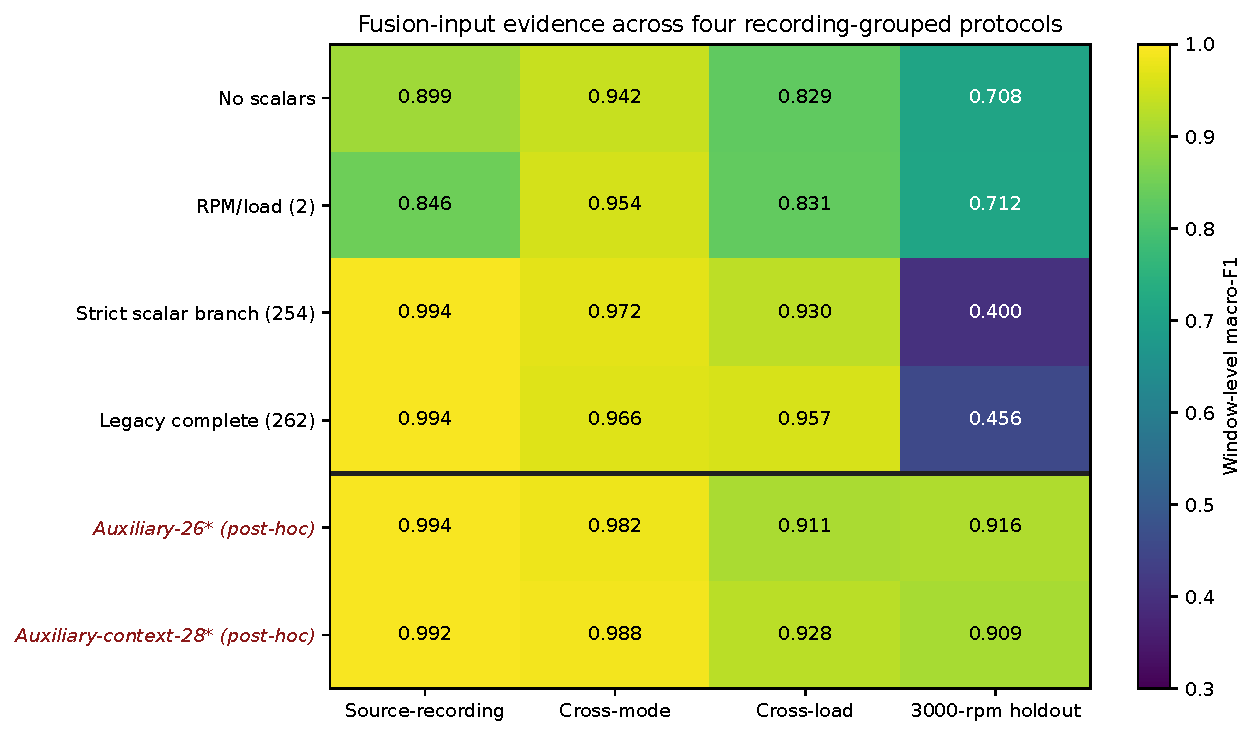
\includegraphics[width=0.96\textwidth]{figures/figure_6_corrected_fusion_heatmap.pdf}
\caption{Complete four-protocol fusion-input comparison. The horizontal separator distinguishes predefined matched configurations from auxiliary-26* and auxiliary-context-28*, which are post-hoc exploratory configurations selected after inspection of the same 3000-rpm holdout. The displayed color range is 0.30--1.00.}
\label{fig:s_protocol_fusion}
\end{figure}

\subsection{Focused 3000-rpm evidence}


\begingroup
\small
\renewcommand{\arraystretch}{1.08}
\begin{longtable}{p{7.0cm} c c c c}
\caption{Per-seed fusion-input results for the 3000-rpm holdout. The auxiliary-26 and auxiliary-context-28 rows are post-hoc exploratory on this same holdout.}\label{tab:s_fusion}\\
\toprule
Configuration & Scalars & Seed & Macro-F1 & Worst recall \\
\midrule
\endfirsthead
\multicolumn{5}{c}{\tablename\ \thetable\ continued}\\
\toprule
Configuration & Scalars & Seed & Macro-F1 & Worst recall \\
\midrule
\endhead
\midrule
\multicolumn{5}{r}{Continued on next page}\\
\endfoot
\bottomrule
\endlastfoot
\multicolumn{5}{l}{\textit{Predefined matched configurations}} \\
Vibration-current; no scalars & 0 & 42 & 0.5599 & 0.2451 \\
Vibration-current; no scalars & 0 & 43 & 0.8027 & 0.6536 \\
Vibration-current; no scalars & 0 & 44 & 0.7366 & 0.4085 \\
Vibration-current; no scalars & 0 & 45 & 0.7792 & 0.3715 \\
Vibration-current; no scalars & 0 & 46 & 0.6623 & 0.4832 \\
Vibration-current + RPM/load & 2 & 42 & 0.7368 & 0.4714 \\
Vibration-current + RPM/load & 2 & 43 & 0.6231 & 0.2793 \\
Vibration-current + RPM/load & 2 & 44 & 0.7605 & 0.4874 \\
Vibration-current + RPM/load & 2 & 45 & 0.7116 & 0.3827 \\
Vibration-current + RPM/load & 2 & 46 & 0.7299 & 0.5154 \\
Strict-254 scalar-branch fusion & 254 & 42 & 0.5236 & 0.0223 \\
Strict-254 scalar-branch fusion & 254 & 43 & 0.3906 & 0.0279 \\
Strict-254 scalar-branch fusion & 254 & 44 & 0.4279 & 0.0321 \\
Strict-254 scalar-branch fusion & 254 & 45 & 0.3166 & 0.0251 \\
Strict-254 scalar-branch fusion & 254 & 46 & 0.3419 & 0.0209 \\
Legacy-262 complete branch & 262 & 42 & 0.4965 & 0.0251 \\
Legacy-262 complete branch & 262 & 43 & 0.5311 & 0.1648 \\
Legacy-262 complete branch & 262 & 44 & 0.4592 & 0.1243 \\
Legacy-262 complete branch & 262 & 45 & 0.3249 & 0.0223 \\
Legacy-262 complete branch & 262 & 46 & 0.4666 & 0.0880 \\
\midrule
\multicolumn{5}{l}{\textit{Post-hoc exploratory configurations on the same holdout}} \\
Vibration-current + auxiliary-26* & 26 & 42 & 0.9121 & 0.8059 \\
Vibration-current + auxiliary-26* & 26 & 43 & 0.9431 & 0.8765 \\
Vibration-current + auxiliary-26* & 26 & 44 & 0.9274 & 0.8715 \\
Vibration-current + auxiliary-26* & 26 & 45 & 0.9209 & 0.8038 \\
Vibration-current + auxiliary-26* & 26 & 46 & 0.8773 & 0.7318 \\
Vibration-current + auxiliary-context-28* & 28 & 42 & 0.8819 & 0.6969 \\
Vibration-current + auxiliary-context-28* & 28 & 43 & 0.8820 & 0.6997 \\
Vibration-current + auxiliary-context-28* & 28 & 44 & 0.9429 & 0.8839 \\
Vibration-current + auxiliary-context-28* & 28 & 45 & 0.9336 & 0.8080 \\
Vibration-current + auxiliary-context-28* & 28 & 46 & 0.9070 & 0.8233 \\
\end{longtable}
\noindent\small * Post-hoc configurations identified after inspection of the same 3000-rpm holdout.
\endgroup


\begin{figure}[H]
\centering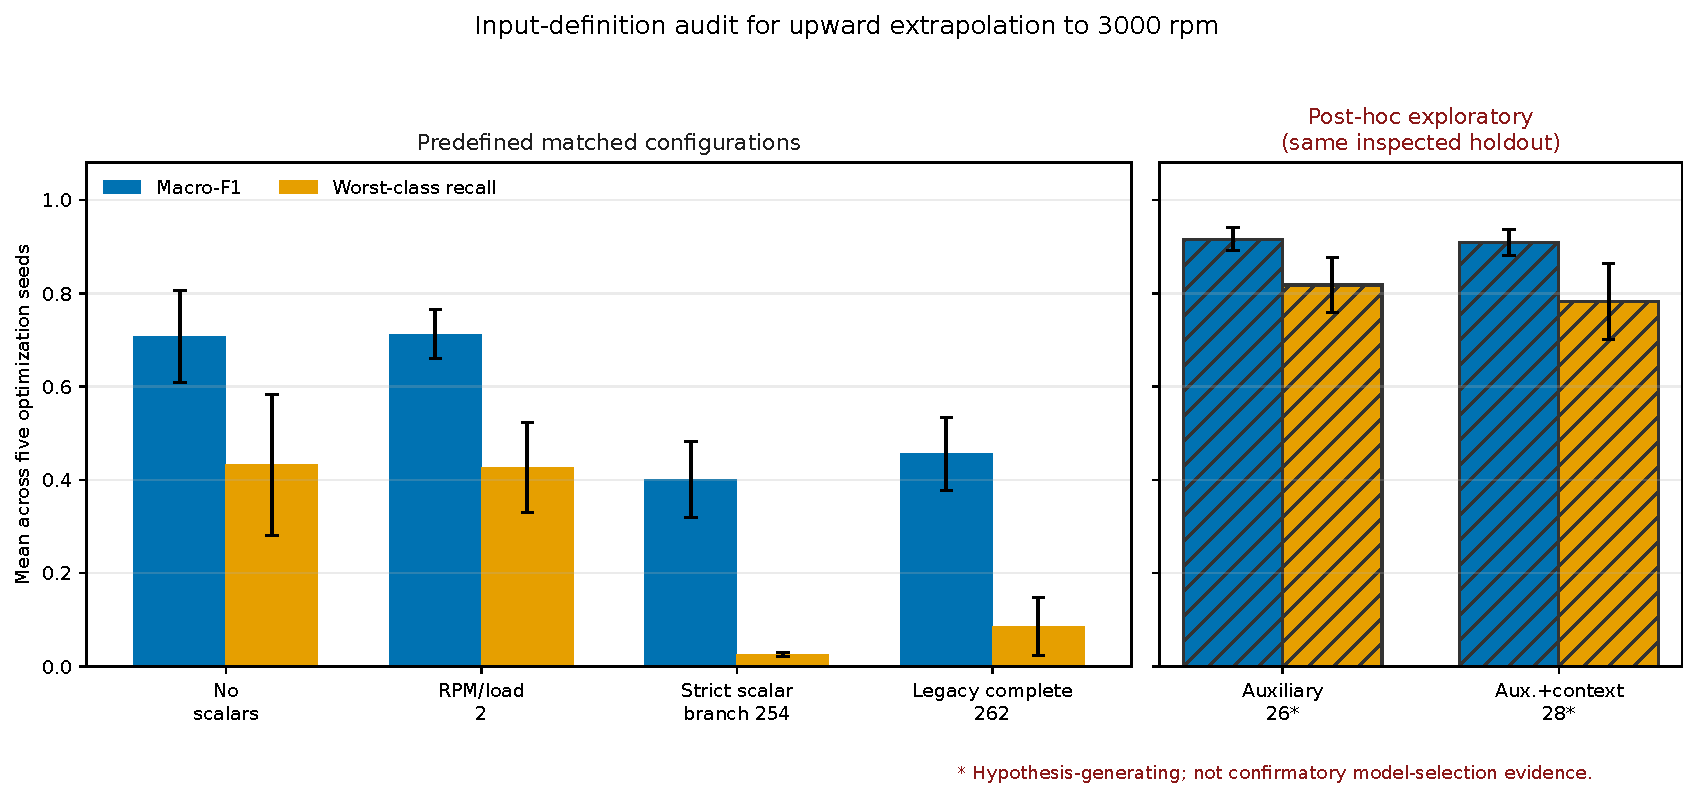
\includegraphics[width=0.94\textwidth]{figures/figure_7_cross_rpm_input_audit.pdf}
\caption{Focused fusion-input audit for upward extrapolation to 3000 rpm. The left panel contains predefined matched configurations; the separate hatched right panel contains post-hoc exploratory configurations identified on the same holdout. Error bars denote standard deviations across five optimization seeds. The right-panel comparison is hypothesis-generating rather than confirmatory.}
\label{fig:s_focused_fusion}
\end{figure}


\begin{table}[H]
\centering
\caption{Recording-level mean-probability aggregation for all fusion-input definitions on the 3000-rpm holdout. Means and standard deviations are calculated across optimization seeds after probabilities have first been aggregated within each recording.}
\label{tab:s_source_fusion}
\small
\resizebox{\textwidth}{!}{%
\begin{tabular}{lcccc}
\toprule
Configuration & Recordings & Recording macro-F1 mean ± SD & Recording worst recall mean ± SD & Evidence status \\
\midrule
Vibration-current; no scalars & 28 & 0.7122 ± 0.1238 & 0.4000 ± 0.2054 & Matched protocol \\
Vibration-current + RPM/load & 28 & 0.7306 ± 0.0917 & 0.4000 ± 0.1369 & Matched protocol \\
Strict-254 scalar-branch fusion & 28 & 0.3660 ± 0.1254 & 0.0000 ± 0.0000 & Matched protocol \\
Legacy-262 complete branch & 28 & 0.3829 ± 0.0917 & 0.0000 ± 0.0000 & Matched protocol \\
\midrule
Vibration-current + auxiliary-26* & 28 & 0.9435 ± 0.0264 & 0.8361 ± 0.0669 & Post-hoc exploratory \\
Vibration-current + auxiliary-context-28* & 28 & 0.9368 ± 0.0513 & 0.8278 ± 0.1439 & Post-hoc exploratory \\
\bottomrule
\end{tabular}}
\vspace{0.3em}\parbox{\textwidth}{\footnotesize * Post-hoc exploratory configuration identified after inspection of the same 3000-rpm holdout.}
\end{table}


\section{Severity and Per-Recording Probability Audits}
The severity analysis is a descriptive, low-cost audit derived from saved source-recording predictions. It was not used for model selection. High- and light-severity fault recordings are evaluated separately; healthy recordings remain ungraded.


\begin{table}[H]
\centering
\caption{Severity-stratified recording-level results on the 3000-rpm holdout. Severity is inferred from the public recording identifier; healthy recordings have no severity grade. Values are means and standard deviations across optimization seeds.}
\label{tab:s_severity}
\small
\renewcommand{\arraystretch}{1.18}
\setlength{\tabcolsep}{3.4pt}
\begin{tabularx}{\textwidth}{>{\raggedright\arraybackslash}X l c >{\centering\arraybackslash}p{0.14\textwidth} >{\centering\arraybackslash}p{0.18\textwidth} >{\raggedright\arraybackslash}p{0.16\textwidth}}
\toprule
Configuration & Severity & Recordings & Accuracy mean $\pm$ SD & Fault macro-F1 mean $\pm$ SD & Evidence status \\
\midrule
Vibration-current; no scalars & High & 12 & 0.6333 ± 0.1728 & 0.5771 ± 0.2166 & Matched protocol \\
Vibration-current; no scalars & Light & 12 & 0.8667 ± 0.1264 & 0.8631 ± 0.1303 & Matched protocol \\
Vibration-current; no scalars & Healthy (ungraded) & 4 & 0.6000 ± 0.3354 & Not applicable (single class) & Matched protocol \\
\midrule
Vibration-current + RPM/load & High & 12 & 0.6667 ± 0.1768 & 0.6272 ± 0.2172 & Matched protocol \\
Vibration-current + RPM/load & Light & 12 & 0.9333 ± 0.0373 & 0.9323 ± 0.0379 & Matched protocol \\
Vibration-current + RPM/load & Healthy (ungraded) & 4 & 0.5000 ± 0.2500 & Not applicable (single class) & Matched protocol \\
\midrule
Strict-254 scalar-branch fusion & High & 12 & 0.4000 ± 0.1369 & 0.3600 ± 0.1710 & Matched protocol \\
Strict-254 scalar-branch fusion & Light & 12 & 0.7500 ± 0.1559 & 0.6929 ± 0.1965 & Matched protocol \\
Strict-254 scalar-branch fusion & Healthy (ungraded) & 4 & 0.0000 ± 0.0000 & Not applicable (single class) & Matched protocol \\
\midrule
Vibration-current + auxiliary-26* & High & 12 & 0.8500 ± 0.0697 & 0.8474 ± 0.0725 & Post-hoc exploratory \\
Vibration-current + auxiliary-26* & Light & 12 & 1.0000 ± 0.0000 & 1.0000 ± 0.0000 & Post-hoc exploratory \\
Vibration-current + auxiliary-26* & Healthy (ungraded) & 4 & 1.0000 ± 0.0000 & Not applicable (single class) & Post-hoc exploratory \\
\bottomrule
\end{tabularx}
\vspace{0.35em}\parbox{\textwidth}{\footnotesize Fault macro-F1 is calculated over the three fault-location classes within each severity subgroup; healthy recordings are reported separately and therefore have no fault macro-F1. * Post-hoc exploratory configuration identified after inspection of the same 3000-rpm holdout.}
\end{table}


Because severity is inferred from recording identifiers and the subgroups are small, these results are descriptive only. The observed differences should not be interpreted as evidence that light-severity faults are intrinsically easier to diagnose than high-severity faults.

\begin{landscape}
\begin{figure}[p]
\centering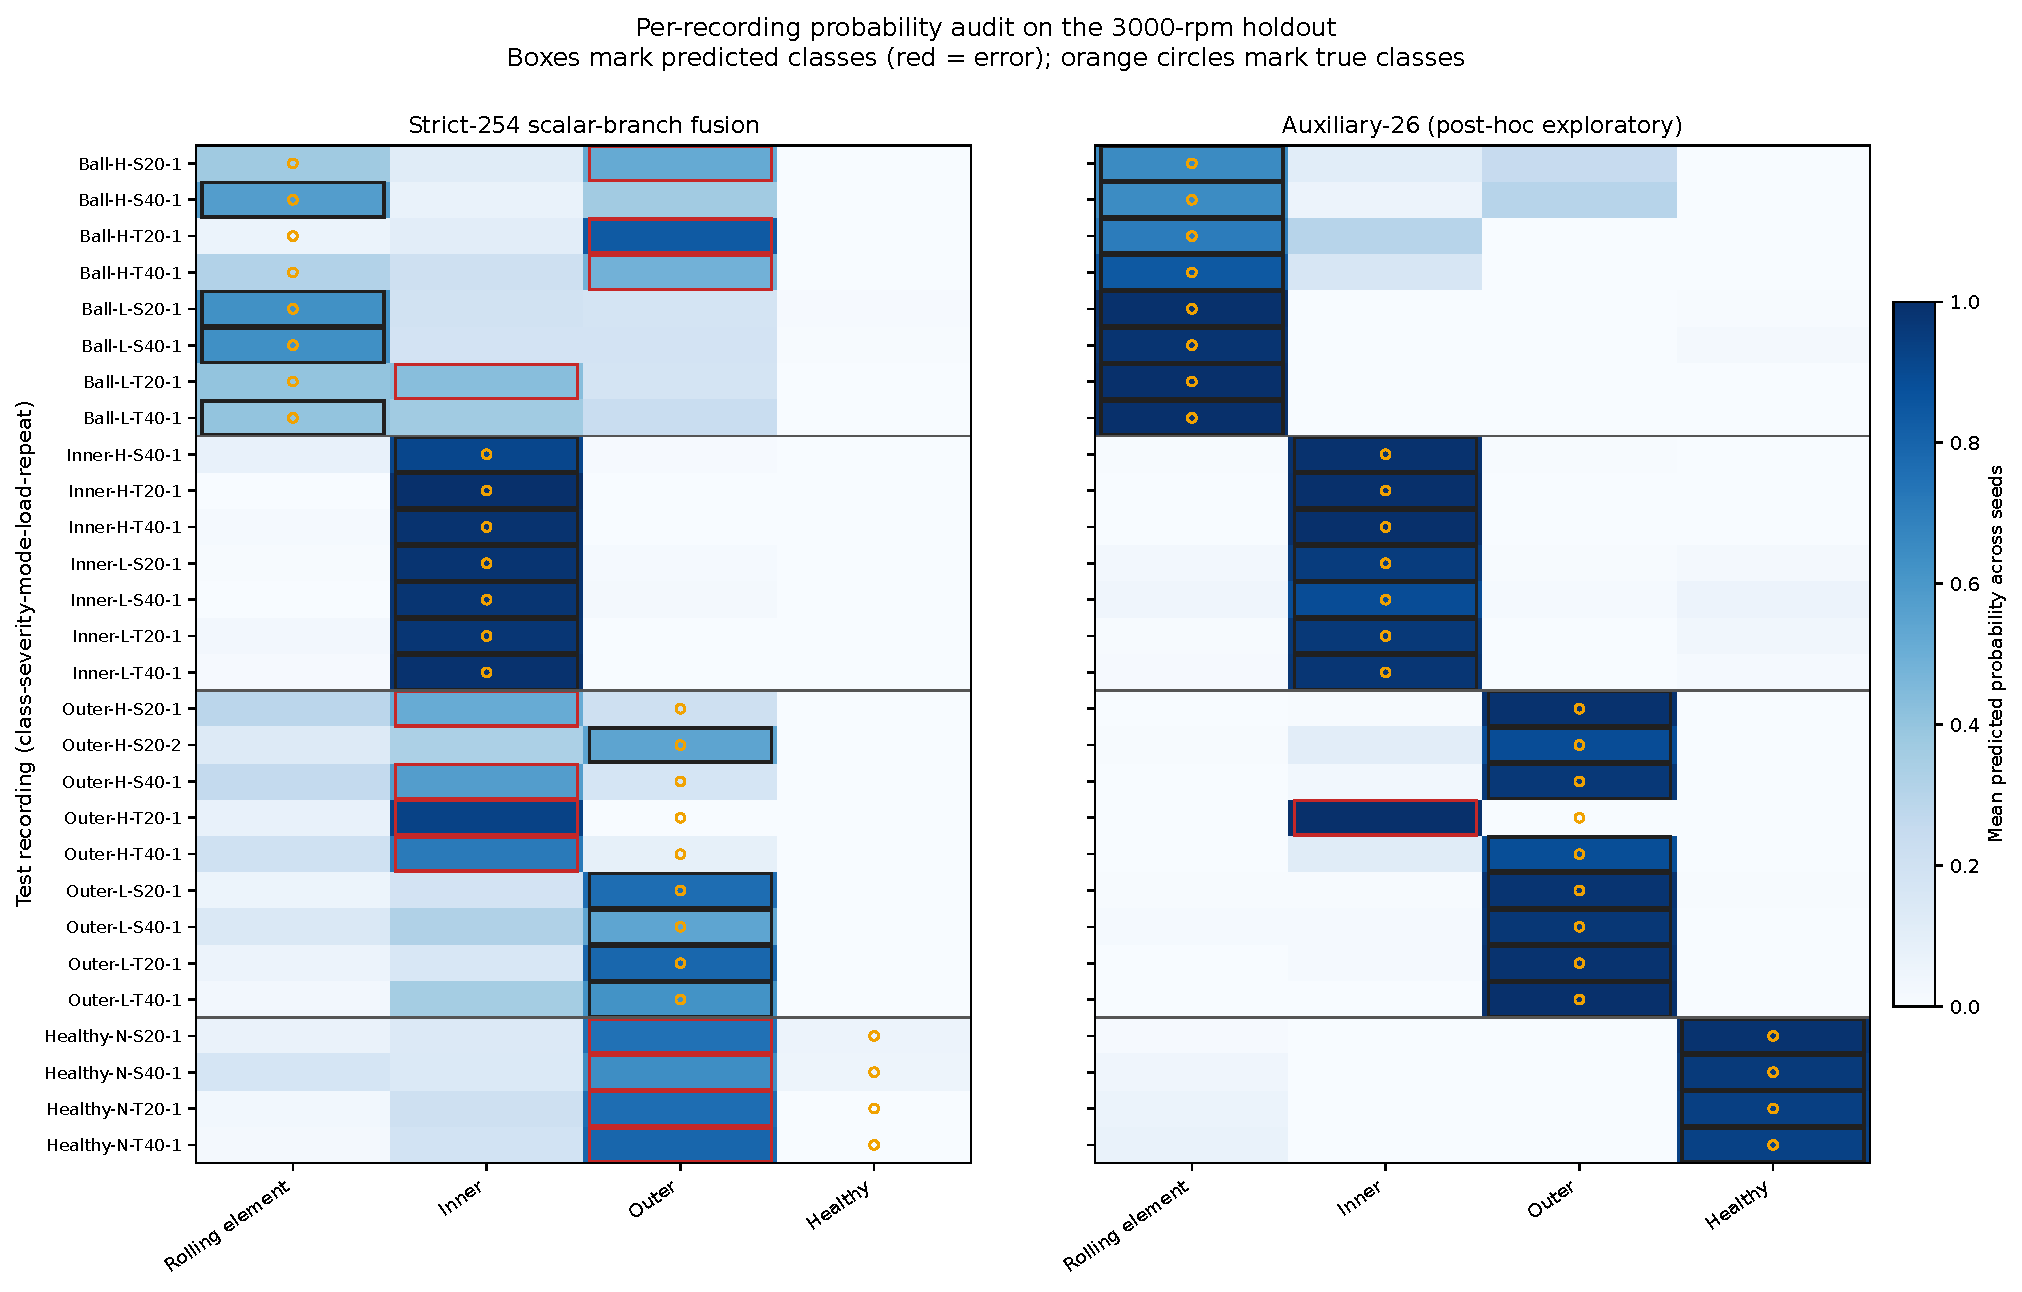
\includegraphics[width=0.96\linewidth,height=0.82\textheight,keepaspectratio]{figures/figure_s3_per_recording_probability.pdf}
\caption{Per-recording class-probability audit on the 3000-rpm holdout, averaged across optimization seeds. Boxes mark the argmax class of the seed-averaged probability vector; red boxes denote errors, and orange circles denote the true class. Publication-facing class labels use ``rolling element''; original recording identifiers retain the dataset prefix ``Ball''. The auxiliary-26 panel is post-hoc exploratory on the same holdout and is shown only to localize the associated recording-level behavior.}
\label{fig:s_recording_probability}
\end{figure}
\end{landscape}

\section{Recording-Level Bootstrap}
Intervals resample complete test recordings within class for 2,000 replicates. They are conditional empirical resampling intervals for the listed finite test recordings and fitted seed. They neither quantify uncertainty for future physical specimens nor convert post-hoc model selection into confirmatory evidence.


\begin{table}[H]
\centering
\caption{Class-stratified recording bootstrap for selected 3000-rpm models. Point estimates are recording-level macro-F1 values obtained after mean-probability aggregation within each recording. Conditional empirical intervals resample complete recordings within class and condition on the listed finite test set and trained seed; they are not intervals for future specimens. The Auxiliary-26 row is post-hoc exploratory, and the intervals do not remove its selection bias.}
\label{tab:s_boot}
\small
\resizebox{\textwidth}{!}{%
\begin{tabular}{lccccc}
\toprule
Model & Evidence status & Seed & Point macro-F1 & 95\% interval & Recordings \\
\midrule
Strict-254 scalar-branch fusion & Matched protocol & 42 & 0.5348 & [0.4242, 0.6244] & 28 \\
Strict-254 scalar-branch fusion & Matched protocol & 43 & 0.2906 & [0.2101, 0.3713] & 28 \\
Strict-254 scalar-branch fusion & Matched protocol & 44 & 0.4478 & [0.3439, 0.5519] & 28 \\
Strict-254 scalar-branch fusion & Matched protocol & 45 & 0.2208 & [0.1540, 0.2955] & 28 \\
Strict-254 scalar-branch fusion & Matched protocol & 46 & 0.3359 & [0.2189, 0.4581] & 28 \\
Auxiliary-26 branch* & Post-hoc exploratory & 42 & 0.9374 & [0.8453, 1.0000] & 28 \\
Auxiliary-26 branch* & Post-hoc exploratory & 43 & 0.9686 & [0.9059, 1.0000] & 28 \\
Auxiliary-26 branch* & Post-hoc exploratory & 44 & 0.9686 & [0.9059, 1.0000] & 28 \\
Auxiliary-26 branch* & Post-hoc exploratory & 45 & 0.9375 & [0.8381, 1.0000] & 28 \\
Auxiliary-26 branch* & Post-hoc exploratory & 46 & 0.9055 & [0.7967, 1.0000] & 28 \\
Raw vibration-current CNN & Matched protocol & 42 & 0.4367 & [0.2922, 0.5515] & 28 \\
Raw vibration-current CNN & Matched protocol & 43 & 0.8888 & [0.7297, 1.0000] & 28 \\
Raw vibration-current CNN & Matched protocol & 44 & 0.8444 & [0.7134, 0.9375] & 28 \\
\bottomrule
\end{tabular}}

\end{table}


\section{Model Architectures and Fixed Hyperparameters}
Table S7 reports the publication-facing settings implemented in the formal benchmark. Classical hyperparameters were fixed before final test evaluation. Neural early stopping and checkpoint selection used only the frozen internal-validation recordings; held-out test recordings did not inform scaling, checkpoint selection, or hyperparameter choice.


\begingroup
\footnotesize
\setlength{\tabcolsep}{3.2pt}
\begin{longtable}{>{\raggedright\arraybackslash}p{2.0cm} >{\raggedright\arraybackslash}p{2.4cm} >{\raggedright\arraybackslash}p{7.4cm} >{\raggedright\arraybackslash}p{3.2cm}}
\caption{Model architectures, preprocessing, and fixed hyperparameters.}\label{tab:s_models}\\
\toprule
Model & Input and preprocessing & Architecture and fixed hyperparameters & Selection and size \\
\midrule
\endfirsthead
\multicolumn{4}{c}{\tablename\ \thetable\ continued}\\
\toprule
Model & Input and preprocessing & Architecture and fixed hyperparameters & Selection and size \\
\midrule
\endhead
\midrule
\multicolumn{4}{r}{Continued on next page}\\
\endfoot
\bottomrule
\endlastfoot
Logistic regression & 254 engineered fields; training-median imputation and StandardScaler & C=1.0; L2 penalty; lbfgs solver; max\_iter=1000 & Fixed before test; 1,020 coefficients/intercepts for 254 inputs and four classes \\
RBF-SVM & 254 engineered fields; training-median imputation and StandardScaler & RBF kernel; C=3.0; gamma=scale & Fixed before test; support-vector count is training-data dependent \\
Random forest & 254 engineered fields; training-median imputation; no scaling & 200 trees; max\_depth=None; min\_samples\_leaf=1; all CPU cores & Fixed before test; trained tree size is data dependent \\
MLP & 254 engineered fields; training-median imputation and StandardScaler & 254->128->4; ReLU; Adam; alpha=1e-4; max\_iter=300 & Fixed before test; 33,156 trainable weights and biases \\
XGBoost & 254 engineered fields; training-median imputation; no scaling & 200 trees; max\_depth=4; learning\_rate=0.05; subsample=0.9; colsample\_bytree=0.9; multiclass log-loss & Fixed before test; trained tree size is data dependent \\
Raw CNN & Six vibration-current channels; 8,192 samples; train-only per-channel z-score & Conv1d 6->32 (kernel 9), batch normalization, ReLU, max-pool 4; Conv1d 32->64 (kernel 7), batch normalization, ReLU, global average pooling; linear 64->4 & Best validation macro-F1; 16,612 trainable parameters \\
TCN & Six vibration-current channels; 8,192 samples; train-only per-channel z-score & Three non-residual dilated Conv1d blocks, width 32, kernel 5, dilations 1/2/4; batch normalization and ReLU; global average pooling; linear 32->4 & Best validation macro-F1; 11,620 trainable parameters \\
Transformer & Six vibration-current channels; 8,192 samples; train-only per-channel z-score & Conv1d token projection 6->64 (kernel 9, stride 8); two encoder layers; d\_model=64; four heads; feed-forward width 128; dropout=0.1; mean pooling; linear 64->4 & Best validation macro-F1; 70,724 trainable parameters \\
Fusion family & Separate three-channel vibration and current sequences plus 0/2/26/28/254/262 scalar definitions; train-only sequence and scalar z-score & Each sequence encoder: Conv1d 3->32 (kernel 9), max-pool 4, Conv1d 32->64 (kernel 7), global average pooling. Scalar MLP d->32->32. Concatenated width 160, sigmoid gate 160->160, classifier 160->64->4, dropout=0.2 & Best validation macro-F1; parameters: 68,420 / 68,452 / 69,220 / 69,284 / 76,516 / 76,772 in the listed scalar order \\
\end{longtable}
\noindent\footnotesize Classical configurations were fixed before final test evaluation. Neural checkpoints were selected by the highest internal-validation macro-F1. Neural models used class-weighted cross-entropy, Adam with learning rate $10^{-3}$, batch size 64, at most 30 epochs, and patience 8; fusion models additionally used weight decay $10^{-4}$.
\endgroup


\section{Reproducibility Notes}
The verified runtime used Python 3.12.13, PyTorch 2.11.0+cu128, and an NVIDIA GeForce RTX 5080. Automated tests cover train-only sequence and scalar standardization, constant channels, missing scalar values, serialization of fitted statistics, source-recording separation across all data roles, raw-file audit integrity, classical source-recording aggregation, and the evidence-status labels applied to exploratory configurations. The software supplement includes frozen split maps, a de-identified window-to-recording index, exact input schemas, compact raw/session audit tables, result tables, and reproduction commands; raw MCC5 signals are not redistributed.

\end{document}
